\documentclass[a4paper,11pt]{article}
\usepackage{graphicx}
\usepackage[utf8]{inputenc}
\usepackage{hyperref}
\usepackage{placeins}
\usepackage[newfloat]{minted}
\usepackage{caption}

\newenvironment{code}{\captionsetup{type=listing}}{}
\SetupFloatingEnvironment{listing}{name=Code Overview}


\hypersetup{
    colorlinks=true,
    linkcolor=blue,
    filecolor=black,      
    urlcolor=blue,
    citecolor=black,
}
\begin{document}

\title{
    \textbf{A Heap or Priority Queue Report.}
}
\author{Adrian Jonsson Sjödin}
\date{Fall 2022}

\maketitle

\section{Task}
\label{task}
The task in this assignment is to create a priority queue using different implementations and determine
the pros and cons of each. The different priority queues to be implemented are listed bellow.
\begin{itemize}
    \item List implementation of priority queue where smaller numbers have higher priority. Make one implementation
    where the cost of adding elements are $\mathcal{O}(1)$ and remove is $\mathcal{O}(n)$, and another where the costs are reversed.
    Benchmark the two implementations and discuss situations where one would be preferred over the other.
    
    \item Priority queue implementing a heap as a linked binary tree where each node holds the element, branches and 
    the total number of elements in the subtree. This to make the tree balanced. You should be able to add and remove elements.
    Also implement a method {\tt push(Integer incr)} that increments the root element by {\tt incr} and then pushes it (by swapping 
    values) to either the left or right branch.

    Set up a benchmark where you first add 64 elements with random values to a heap. The run a sequence of push operations 
    where you increment a by a random number ($\in[10,20]$). Collect some statistics on how deep the push operations need to go.
    
    Change the add method so that it also returns the depth. Run the same benchmark as above but now collect statistics on the 
    add method.

    \item Priority queue implementing a heap using an array. Benchmark the array implementation and see how it compares to the 
     linked list implementation.

\end{itemize}

\section{Method \& Theory}
\label{method}
\subsection{List Priority Queue with constant add method}
\label{ListQueue}
We started with implementing the linked list priority queue who had a constant time complexity of adding items 
to the queue and a time complexity of $\mathcal{O}(n)$ to remove the minimum element. 

Achieving a constant time for 
adding elements was done by having a pointer to the last element in the list which we then could jus re-point to 
the new element and also let the previous last point to the new element. These steps takes a constant time regardless 
of how long the queue is, thus giving us a time complexity of $\mathcal{O}(n)$. The code for {\tt add} can be seen
in code overview \ref{code:ListQueueAdd}.

The elements in the list are not sorted since we just add new elements to the end of the list each time. This means 
that when we want to retrieve and remove the minimum element in the queue it could be placed anywhere in it and 
we need to traverse the list from the first element all the way to the last. The time complexity of 
removing one element will thus be $\mathcal{O}(n)$ for best case, worse case and average case. 

Actually removing the minimum element is achieved by having a pointer that looks at the current node in the list and 
loop through the whole list until we reach the next to last node in the list, and for each node check if it is 
less than the the current min. If it is we save that node's value as well as a pointer to the previous node and the 
node after. When we have looped through the whole list min will be the value of the minimum node and we will have 
a pointer to the node before and after. We then just make the node before point to the node after thus removing the 
found minimum node from the list, and lastly return the minimum value. The code for this can be seen in code 
overview \ref{code:ListQueueRemove}.

\subsection{List Priority Queue with constant remove method}
\label{QueueList}
The second linked list priority queue we implemented was one where we sorted the items when we added them to the queue
making sure that the smallest value was always at the front of the list, followed by successively larger values. 
This way we could achieve a constant time complexity when we remove the minimum value since it is always at the front 
of the queue and simply re-pointing {\tt first} to point to {\tt first.next} is a constant time operation. The code 
for this can be seen in code overview \ref{code:QueueListRemove}.

For the add method we had to make sure that we always insert it in the queue so that the element before it is smaller 
and the element behind is larger. This means that we only need to make one comparison if we're lucky and the 
element we want to add is smaller than the first element in the queue, giving us a time complexity of $\mathcal{O}(1)$
in the best case. On the other hand we could be unlucky and it is larger than any of the elements in the queue giving 
us a time complexity of $\mathcal{O}(n)$ in the worst case. On average though we will have a time complexity of 
$\mathcal{O}(\frac{n}{2})=\mathcal{O}(n)$ which is still a linear time complexity to add but should be faster than 
the remove method described in section \ref{ListQueue}. 

The way we do this is quite simple. First we check if the queue is empty or if the item we want to add is smaller 
than first. If it is we simply add it in the first position, let {\tt first} point to it and let it point to the 
rest of the queue. If it is not one of those we start looping through the array until we find the position where 
we want to insert it, insert it and and let it point to the following nodes in in the queue. The code for this can 
be seen in code overview \ref{code:QueueListAdd}.

\subsection{Priority Tree}
This was the hardest method to implement since it required one to use recursive method calls. We needed to implement 
a tree structure where the root was the element with the lowest priority and each branch was successively larger. 
That is if the root had the highest priority then either the left or right branch should be the second highest 
and then the third highest and so on. This meant that we needed to be able to push nodes further down the tree 
to make room for smaller items. We also needed to make sure the tree was balanced and this we did by letting each node hold the value of 
how many branches it had and always adding the new node to the node who had the least branches. The way to implement 
this is described in the assignment instructions so I won't go through that here but for those interested the 
code implementation can be seen in code overview \ref{code:TreeAdd}.

We also want to be able to retrieve the item with the highest priority. This will always be the root but after 
retrieving it we also need to remove it and move the second highest priority up to be the new root, and in turn 
keep moving up nodes to fill the empty spots. How this is implemented is once again described in the assignment 
instructions but for those interested the code can be seen in code overview \ref{code:TreeRemove}.

Finally we wanted to implement a method that simply took the root and changed it's priority with a specified 
amount and then pushed it down the tree to a fitting place. This so that we don't need to first run remove to operate 
on the item before pushing it back to the tree, which would require more execution time than to simply operate 
on it when it is still in the tree and just push it down when we're finished. 

We used the {\tt remove} method as a basis since it already almost does what we want. We simply had to make some 
adjustments so that no node was removed and make a small private helper method that swaps the contents of two 
nodes. The code for this method can be seen in code overview \ref{code:TreePush}.

\subsection{Array Heap}
The last task was to implement the Array Heap. It takes the binary tree heap and convert it to an array form which 
makes it so that we can have a complete binary tree. The way it does so is by clever manipulation of how items are 
added to the queue. A node who has it position at index $n$ will have it's left branch at index $n\cdot 2 +1$
and it's right node at $n \cdot 2 + 2$. The root will always be at index 0 so the root's left child will be at 
position 1 and it's right child at position 2. The left child will in turn be a parent for a left child at index 
3 and a right child at index 4 and so on. 

If we have a queue that is filled until index $k$ and want to add a new item so will we first add it at index $k+1$.
We then compare that items priority against the priority of its parent and if it has a higher priority we swap them.
We let it bubble up through the array like this until either it has no more parents to compare against (in which 
case it has become the new root) or the parent has a higher priority. We can easily get the parent index from the
child index by simply taking $(childIndex -1)/2$ and in turn then retrieve the parent's priority. The code for the 
add method can be seen in code overview \ref{code:ArrayAdd}.

When removing, the item with highest priority will as stated be the root at index 0. We will remove it and then let 
the last item in the queue (item at index $k$) become the new root. There is of course a big chance that this is 
not the item with the highest priority in the queue so we have to let this new root sink down in the array. This is 
done by utilizing a while loop that runs until the item at the current index no longer have a left child or we break it.
In the while loop we then first save the index of the left child. We also check
if the right child has an even higher priority than the left child and save that index instead if it does. After 
this we check if the new root has a higher priority than the child at the saved index. If it does then it is in 
the correct place in the queue and we can break the while loop. If it is lower they swap places and we set index 
to be saved index and repeat the process. This way the new root will sink down to it's appropriate spot. The code
for this can be seen in code overview \ref{code:ArrayRemove}.

\section{Result}
Figure \ref{fig:ListQueueRemove} shows how the time for the remove operation described in section \ref{ListQueue} changes
with regards to the size of the queue. The graph shows the minimum time taken for one remove operation from a queue
of size $n$ where the minimum time is the minimum from $1000$ loops where the queue is filled with the same random 
elements each time.
\begin{figure}[h!]
    \centering
        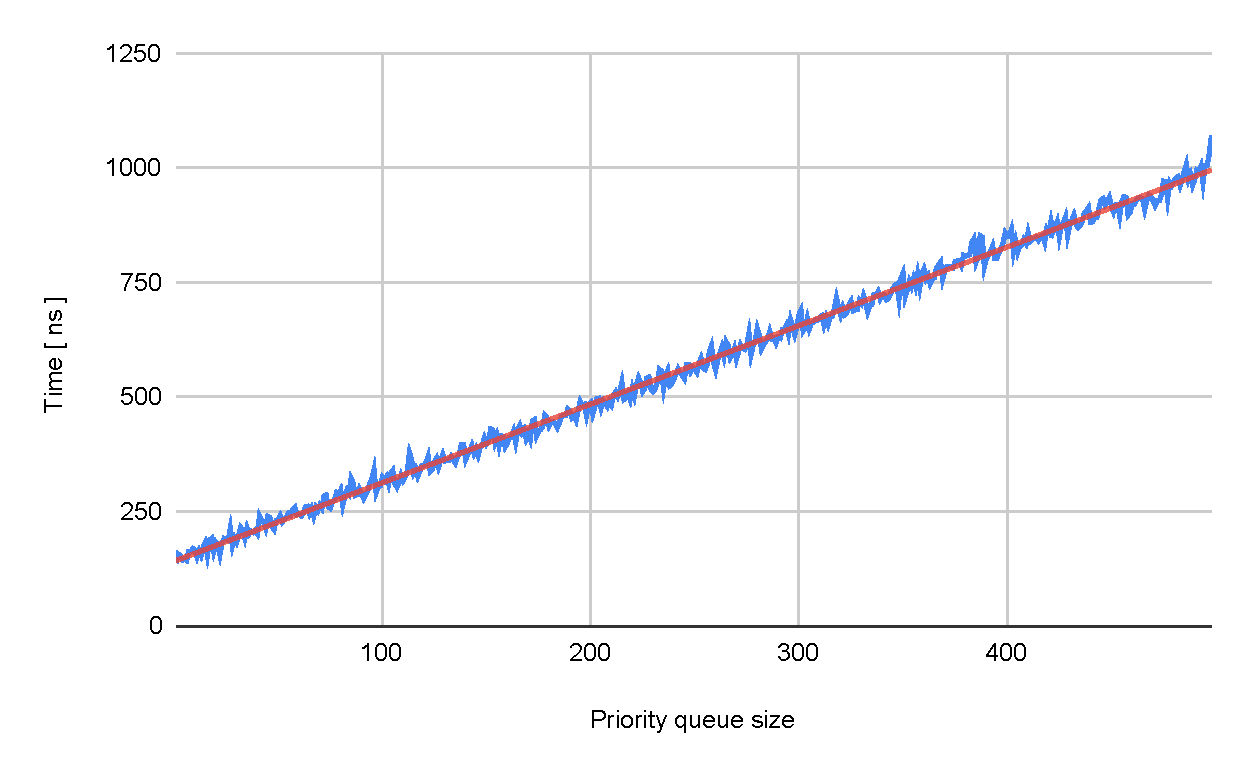
\includegraphics[width=\textwidth]{ListQueueRemove.pdf}
    \caption{{\tt remove()} for list priority queue with constant add method}
    \label{fig:ListQueueRemove}
\end{figure}

Figure \ref{fig:QueueListAdd} shows how the time for the add operation described in section \ref{QueueList} changes
with regards to the size of the queue. The graph shows the minimum time taken for one add operation from a queue
of size $n$ where the minimum time is the minimum from $1000$ loops where the queue is filled with the same random 
elements each time.
\begin{figure}[h!]
    \centering
        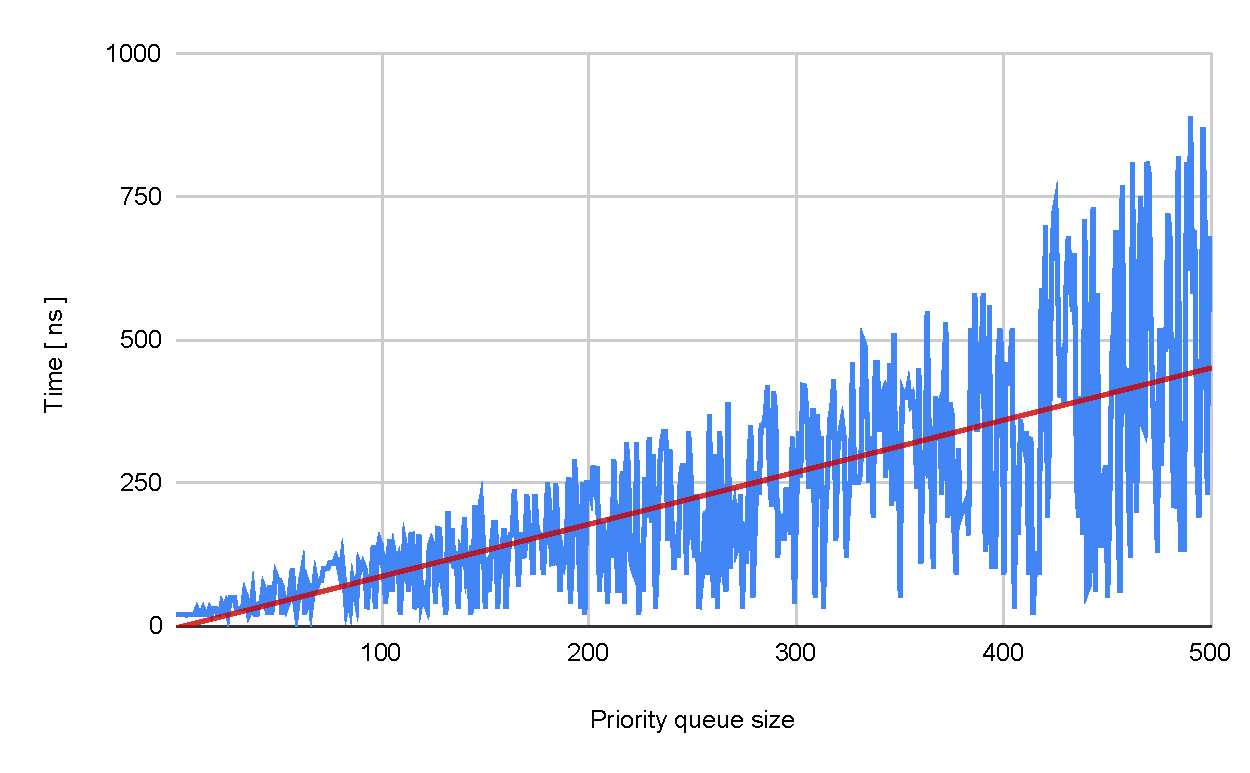
\includegraphics[width=\textwidth]{QueueListAdd.pdf}
        \caption{{\tt add(...)} for list priority queue with constant remove method}
        \label{fig:QueueListAdd}
    
\end{figure}

In table \ref{tab:tree} we see how deep the push method had to go in a three with 64 nodes when we want to change 
the priority of the root. We also see how deep the add method had to go when adding new nodes to a tree with 64 
nodes.
\begin{table}[h!]
    \begin{center}
        \begin{tabular}{|c|c|c|c|}
            \hline
            \textbf{push} & \textbf{Depth} & \textbf{add} & \textbf{Depth}\\
            \hline
             12        & 2    & 10    & 6                           \\
             17        & 3    & 19    & 6                           \\
             17        & 4    & 16    & 6                           \\
             12        & 3    & 10    & 3                           \\
             14        & 4    & 17    & 6                           \\
             20        & 3    & 10    & 3                           \\
             11        & 4    & 14    & 6                           \\
             15        & 3    & 11    & 6                           \\
             15        & 4    & 20    & 6                           \\
             13        & 4    & 19    & 6                           \\
             12        & 5    & 15    & 6                           \\
             13        & 4    & 11    & 6                           \\
             20        & 5    & 15    & 6                           \\
             13        & 4    & 17    & 6                           \\
             17        & 2    & 10    & 6                           \\
             17        & 5    & 16    & 6                           \\
             14         &4    & 11    & 6                           \\
             17         &5    & 19    & 5                           \\
             17         &5    & 11    & 6                           \\
             17         &5    & 11    & 4                           \\
            \hline
        \end{tabular}
        \caption{Benchmark for how deep the push and add method needed to go in the tree}
        \label{tab:tree}
    \end{center}
\end{table}
\FloatBarrier
\section{Discussion}

We see in figure \ref{fig:ListQueueRemove} that the remove method described in section \ref{ListQueue} has the 
expected time complexity of $\mathcal{O}(n)$ We also see in figure \ref{fig:QueueListAdd} that the add method 
described in section \ref{QueueList} have on average the expected time complexity of $\mathcal{O}(n)$. The graph 
in figure \ref{fig:QueueListAdd} might not be as smooth but that is expected since we push random values and 
sometimes we get lucky which will give us a low time, while sometimes we get unlucky which will give us a high
time. But if we look at the red trend line we see that about half lies above it and half below it, giving us that
it is a linear time increase on average. 

We also see that the add method is faster than the remove method which is expected since it doesn't have to 
traverse the whole queue each time. This coupled with the fact that the remove method for this implementation 
of a priority queue is constant makes it a better choice than the other list implementation.

The binary tree implementation on the other hand should have a time complexity of $\mathcal{O}(log(n))$ for 
both add and remove. This since we will only need to make $d$ comparisons (where $d$ is the depth of the tree) 
when adding or removing an element, and since it is a binary tree so will $d$ be $log(n)$, where $n$ is the total 
amount of nodes in the tree. 

While the binary tree heap offers on general a better time complexity of $\mathcal{O}(log(n))$ than either of 
the linked list priority queues it still has it drawbacks. For one it still utilizes a nodes with pointer making
for long access time when fetching the memory address and traversing the tree. Furthermore if we run a sequence of 
remove operations the tree could become unbalanced. 

Regarding the push method in the priority tree we see in table \ref{tab:tree} that it doesn't have to go as deep 
as the add method. The reason why we would want a push method is as stated so that we don't first have to remove
the root which would incur a time cost of $\mathcal{O}(log(n))$ for pushing up a new root and then another time 
cost of $\mathcal{O}(log(n))$ when adding the item back to the tree. Using the push method we can keep the cost down to 
just one $\mathcal{O}(log(n))$ operation.

Finally we have the array implementation of the binary tree heap. This is the method that is the clear winner 
since it has the same advantage as the tree implementation of being of time complexity $\mathcal{O}(log(n))$
while not having the drawback of relatively cost memory access operations as compared to the quick read operation 
of an array index, nor being able to become unbalanced when removing elements. It still have one drawback though 
and that is that the heap could become full, but this can be minimized since you can specify how big you want 
the heap to be when it is initialized and knowing what the heap will be used for can give an indication for how 
big of a heap is required. And even if it would become full we know from previous assignment that the amortized 
cost of expanding it is $\mathcal{O}(log(n))$. 

Unfortunately I couldn't get my benchmark for the array heap class to work. I suspect that the JVM or compliler 
does some kind of optimization since the more loops I ran I just got closer to having {\tt add} and 
{\tt remove} take constant time, bottoming out on 20 ns each regardless of queue size. I have however tested the 
queue extensively with adding elements with random priority and printing it and all parents are in the correct order 
and I always get the element with the highest priority when running {\tt remove}.  


\newpage
\FloatBarrier
\section*{Code}
All the code can be found here: \href{https://github.com/adrian-jonsson-sjoedin/ID1021-AlgoData/tree/main/Tasks/Priority-Queues/src}{GitHub}

\begin{code}
    \captionof{listing}{$\mathcal{O}(n)$ {\tt add(Integer item)} method }
    \label{code:ListQueueAdd}
    \begin{minted}{java}
public void add(Integer item) {
Node newNode = new Node(item, null);
if (this.first == null)
    this.first = newNode;
if (this.last != null)
    this.last.next = newNode;
this.last = newNode;
}
\end{minted}
\end{code}

\begin{code}
    \captionof{listing}{$\mathcal{O}(n)$ {\tt remove()} method}
    \label{code:ListQueueRemove}
    \begin{minted}{java}
public Integer remove() {
    if (this.first == null) {
        System.out.println("remove(): queue is empty");
        return null;
    }
    if (this.first.next == null) {
        int min = this.first.item;
        this.first = null;
        return min;
    }
    Node current = this.first;
    int min = Integer.MAX_VALUE;
    Node beforeMin = null;
    boolean isFirst = false;
    Node prev = null;
    Node after = null;
    while (current != null && current.next != null) {
        if (current.item < min) {
            if (current == this.first) {
                isFirst = true;
                min = current.item;
            } else {
                min = current.item;
                beforeMin = prev;
                after = current.next;
                isFirst = false;
            }
        }
        prev = current;
        current = current.next;
    }
    if (isFirst) {
        this.first = this.first.next;
    } else {
        beforeMin.next = after;
    }
    return min;
}

    \end{minted}
\end{code}

\begin{code}
    \captionof{listing}{$\mathcal{O}(1)$ {\tt remove()} method}
    \label{code:QueueListRemove}
    \begin{minted}{java}
public Integer remove() {
    if (this.first == null) {
        System.out.println("Queue is empty. Nothing to retrieve");
        return null;
    }
    int retrievedItem = this.first.item;
    this.first = this.first.next;
    return retrievedItem;
}
    \end{minted}
\end{code}

\begin{code}
    \captionof{listing}{$\mathcal{O}(n)$ {\tt add(Integer item)} method}
    \label{code:QueueListAdd}
    \begin{minted}{java}
public void add(Integer item) {
    if (this.first == null) { // add node first if queue is empty
        this.first = new Node(item, null);
        return;
    }
    // if head of queue has lower priority than item
    Node current = this.first;
    Node after;
    if (item < current.item) {
        Node newNode = new Node(item, current);
        this.first = newNode;
    } else {
        while (current.next != null && current.next.item < item) {
            current = current.next;
        }
        after = current.next;
        current.next = new Node(item, after);
    }
}
    \end{minted}
\end{code}

\begin{code}
    \captionof{listing}{$\mathcal{O}(log(n))$ {\tt add(int priority, T item)} method}
    \label{code:TreeAdd}
    \begin{minted}{java}
public int add(int priority, T item) {
int depth = 0;
if (root == null) {
    root = new Node(priority, item, 1);
} else {
    depth = root.add(priority, item, 1);
}
return depth;
}
private int add(int prio, T item, int depth) {
    if (this.priority == prio) {
        this.item = item;
        return depth;
    }
    // we want to move the item and prio of the current node down if the item we
    // want to add has lower priority than the node we're in
    if (prio < this.priority) {
        int tempPriority = this.priority;
        T tempItem = this.item;
        this.priority = prio;
        this.item = item;
        prio = tempPriority;
        item = tempItem;
    }
    this.size++;
    if (this.left == null) {
        this.left = new Node(prio, item, 1);
        return depth;
    } else if (this.right == null) {
        this.right = new Node(prio, item, 1);
        return depth;
    } else if (this.right.size < this.left.size) {
        return this.right.add(prio, item, depth + 1);
    } else {
        return this.left.add(prio, item, depth + 1);
    }
}
    \end{minted}
\end{code}
\newpage
\begin{code}
    \captionof{listing}{$\mathcal{O}(log(n))$ {\tt remove()} method}
    \label{code:TreeRemove}
    \begin{minted}{java}
public int remove() {
    if (root == null) {
        System.out.println("Heap is empty");
        return -1;
    } else if (root.left == null && root.right == null) {
        int oldRootToBeReturned = (int) this.root.priority;
        root = null;
        return oldRootToBeReturned;
    } else {
        int oldRootToBeReturned = (int) this.root.priority;
        root.remove();
        return oldRootToBeReturned;
    }
}
private Node remove() {
    // if the left branch is empty we promote the right branch to root.
    if (this.left == null) {
        this.priority = this.right.priority;
        this.item = this.right.item;
        this.right = null;
        this.size--;
        return this;
    }
    // if the right branch is empty we promote the left branch to root
    if (this.right == null) {
        this.priority = this.left.priority;
        this.item = this.left.item;
        this.left = null;
        this.size--;
        return this;
    }
    if (this.left.priority < this.right.priority) {
        this.priority = this.left.priority;
        this.item = this.left.item;
        this.size--;
        if (this.left.size == 1) {
            this.left = null;
        } else {
            this.left = this.left.remove();
        }
        return this;
    } else {
        this.priority = this.right.priority;
        this.item = this.right.item;
        this.size--;
        if (this.right.size == 1) {
            this.right = null;
        } else {
            this.right = this.right.remove();
        }
    }
    return this;
}
    \end{minted}
\end{code}

\begin{code}
    \captionof{listing}{The {\tt push(int increment)} method}
    \label{code:TreePush}
    \begin{minted}{java}
public int push(int increment) {
    this.root.priority += increment;
    Node current = this.root;
    return push(this.root.priority, current, 0);
} 
private int push(int newRootValue, Node current, int depth) {
    if (current.left == null) {
        if (newRootValue < current.right.priority) {
            return depth;
        } else if (current.left.priority < newRootValue) {
            depth++;
            swapMinNodeUp(current, current.right);
        }
        if (current.right.size != 1) {
            depth = push(newRootValue, current.right, depth);
        }
    }
    if (current.right == null) {
        if (current.left.priority > newRootValue) {
            return depth;
        } else if (current.left.priority < newRootValue) {
            depth++;
            swapMinNodeUp(current, current.left);
        }
        if (current.left.priority != 1) {
            depth = push(newRootValue, current.left, depth);
        }
    }
    if (current.left.priority > current.right.priority) {
        if (current.right.priority > newRootValue) {
            return depth;
        } else if (current.right.priority < newRootValue) {
            depth++;
            swapMinNodeUp(current, current.right);
        }
        if (current.right.size != 1) {
            depth = push(newRootValue, current.right, depth);
        }
    } else {
        if (current.left.priority > newRootValue) {
            return depth;
        } else if (current.left.priority < newRootValue) {
            depth++;
            swapMinNodeUp(current, current.left);
        }
        if (current.left.size != 1) {
            depth = push(newRootValue, current.left, depth);
        }
    }
    return depth;
}
    \end{minted}
\end{code}

\begin{code}
    \captionof{listing}{Array Heap {\tt add(int item)} method}
    \label{code:ArrayAdd}
    \begin{minted}{java}
public void add(int item) {
    if (this.itemsInQueue == maxSize) {
        System.out.println("Heap is full. Can't add item");
        return;
    } // itemsInQueue will always be a value that gives an index where there is
      // nothing inserted yet
    this.priorityQueue[this.itemsInQueue] = item;
    this.itemsInQueue++;
    bubble();
}
    \end{minted}
\end{code}
\begin{code}
    \captionof{listing}{Array Heap {\tt remove()} method}
    \label{code:ArrayRemove}
    \begin{minted}{java}
public int remove() {
    if (this.itemsInQueue == 0) {
        System.out.println("Heap is empty");
        throw new NoSuchElementException();
    }
    int returnElement = this.priorityQueue[0];
    this.priorityQueue[0] = this.priorityQueue[this.itemsInQueue - 1]; // set last element as root
    this.itemsInQueue--;
    sink(); // let the new root sink down
    return returnElement;
}
private void sink() {
    int index = 0; // where we had the old root
    while (hasLeftChild(index)) {
        int smallestChildIndex = getLeftChildIndex(index);
        if (hasRightChild(index) && rightChildValue(index) < leftChildValue(index)) {
            smallestChildIndex = getRightChildIndex(index);
        }
        if (this.priorityQueue[index] < priorityQueue[smallestChildIndex]) {
            break;
        } else {
            swapElements(index, smallestChildIndex);
        }
        index = smallestChildIndex;
    }
}
    \end{minted}
\end{code}

\end{document}
